\documentclass[10pt]{article}
\usepackage{graphicx,heqn,makeidx,epsfig}
%\usepackage{lscape} 
%\usepackage{ae,aecompl} 
%\linespread{1.6}

%override `article' default page layout
\evensidemargin 0.0in 
\oddsidemargin 0.0in
\textwidth 6.5in 
\textheight 9.0in 

\makeindex

\begin{document}

\title{Alice in Meq Land \\
or, thinking the unthinkable} 

\author{A.G. Willis\\ National Research Council of Canada\\ Dominion Radio Astrophysical Observatory\\
Penticton, BC, Canada V2A 6K3\\
\emph{Tony.Willis@nrc-cnrc.gc.ca}}          

\maketitle
\tableofcontents
\pagebreak

\begin{abstract}
This note attempts to give a simplified overview of MeqTrees (short
for `Measurement Equation Trees'), especially how they are built
and how they work. We shall do so by constructing a very simple
MeqTree that solves for polynomial coefficients that describe a 
two-dimensional surface. 
\end{abstract}

\section{Building a Meqtree}
Oleg Smirnov's \cite{smirnov} document gives a detailed description
of MeqTrees and their inner workings. Here we attempt to give a simplified,
yet practical example of constructing an elementary MeqTree to do a simple 
calculation. Figure ~\ref{fig:tree} shows the MeqTree that we will
construct for the purposes of this exercise. We shall show how this
tree is built with an aips++ glish script and show the contents of the
various nodes during or after completion of the calculation. During
the course of this discussion we shall refer to sections of the
glish script by numberings such as {\tt \#\#\#\# 1}. Look for the
corresponding label in the script. The script starts on the next page
and is displayed in the standard Unix {\tt font used for computer
program text}.

We first create a MeqServer object {\tt \#\#\#\# 1}. The MeqServer
object does the work of managing the nodes and their connections.
Its internal workings are presently beyond the scope of this document.
Much of the remainder of the script consists of commands to the
MeqServer to do various operations such as create a new node, `Create.Node',
or execute a request, `Node.Execute'.

MeqTrees consist of MeqNodes of various kinds and the connections 
between these nodes. After we have created a MeqServer we can begin
to create some nodes. 

The first object we create is a MeqPolc (see
the part of the script beginning with {\tt \#\#\#\# 2}).
A MeqPolc represents a polynomial over some rectangular domain in $x$ and
$y$. Nominally, in the world of the Meq $x$ and `Freq' are
interchangeable as is $y$ and `Time'.

We are going to fit a function of the form a + b$x$ +c$y$ +d$xy$ to a
two dimensional surface so we create a 2$x$2 array to store the final
coefficients and make a guess that $a$ will have a value of 1.

Since we are going to fit a function over a surface we need to
specify the bounds of the surface. We do this by creating a  {\tt domain}
(see section 2.2.2 of Oleg Smirnov's \cite{smirnov} document) which
covers the range 0 through 1 in both $x$ and $y$ - see {\tt \#\#\#\# 3}. 
In the {\tt meq.domain} method call, the first two numbers define
the frequency domain.

The actual MeqPolc can now be constructed from a combination of the 
coefficients array and the domain bounds - see  {\tt \#\#\#\# 4}.

%\vspace{0.3cm}
\begin{figure}
{\par\centering
\resizebox*{0.8\columnwidth}{!}{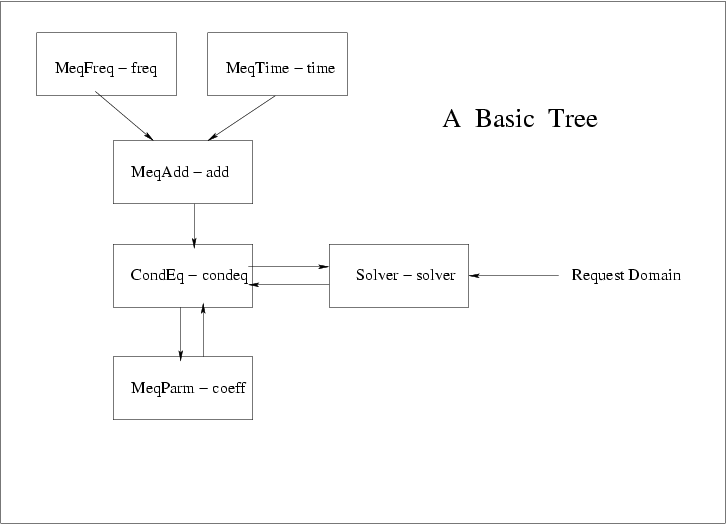
\includegraphics{Figures/tree}}
\par}
\caption {A simple MeqTree consisting of a Solver, a CondEq
and the CondEq's children. This tree is discussed in detail in the
text. The nodes in the tree are labeled both with their generic
Meq type and the specific names that they are given in the glish 
script.} 
\label{fig:tree}
\end{figure}

\begin{figure}
  \centering
  \begin{minipage}[c]{0.5\textwidth}
     \centering 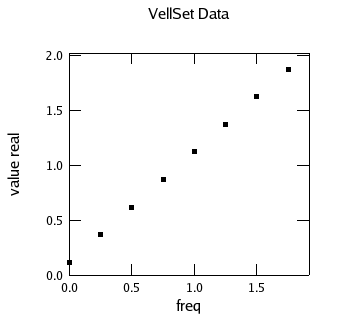
\includegraphics[width=2.5in]{Figures/freq}
  \end{minipage}%
  \begin{minipage}[c]{0.5\textwidth}
     \centering 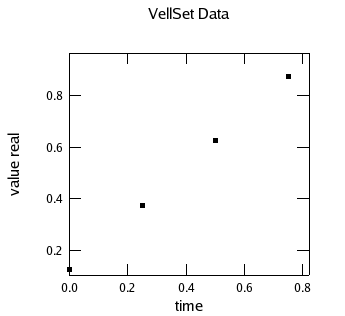
\includegraphics[width=2.5in]{Figures/time}
  \end{minipage}
  \caption {The contents of the MeqFreq (left) and MeqTime (right) objects.
  They are simple one-dimensional arrays.} 
  \label{fig:freq}
\end{figure}


%\pagebreak
%\begin{scriptsize}
\begin{verbatim}
################ glish script to make a simple MeqTree ####################

#### 1
# instantiate a 'Meq' server
# the server does the work of creating nodes etc
# this function call is simplified a bit for pedagogical purposes
mqs := meq.server();

# now create a simple MeqTree

#### 2
# first create 2x2 polc
# The 'polc' array will be used to store the coefficients a,b,c,d
# for the polynomial fit in x and y (a +bx +cy +dxy) that we will do below
polc_array := array(as_double(0),2,2) 
polc_array[1,1] := as_double(1)
# initially we have guessed the coefficients a=1, and b,c,d = 0

#### 3
# we now create a time-frequency 'domain' with range 0 to 2 in frequency and
# 0 to 1 in time 
test_domain := meq.domain(0,2,0,1);

#### 4
# create an actual MeqPolc from the polc_array and the domain specification
meq_polc := meq.polc(polc_array,domain=test_domain)
                                                                                
#### 5
# we now create a leaf called 'coeff' which is of type MeqParm and contains
# the MeqPolc we created previously. It has no children
mqs.meq('Create.Node',meq.parm('coeff',meq_polc,groups='Parm'));

#### 6
# now create a leaf MeqFreq node called 'freq' which has no children
mqs.meq('Create.Node',meq.node('MeqFreq','freq'));

#### 7
# create a leaf MeqTime node called 'time' which has no children
mqs.meq('Create.Node',meq.node('MeqTime','time'));

#### 8
# create a MeqAdd node called 'add' which has the children 'freq' and
# 'time'. As its name indicates it will add the contents of 'freq' and
# 'time' together.
mqs.meq('Create.Node',meq.node('MeqAdd','add',children="freq time"));

#### 9
# create a MeqCondeq node called 'condeq'. A MeqCondeq compares the 
# contents of the 'add' and 'coeff' nodes 
mqs.meq('Create.Node',meq.node('MeqCondeq','condeq',children="add coeff"));

#### 10
# now define parameters for the solver - there are several parameters
rec := meq.node('MeqSolver','solver',children="condeq");
# specify that we are to iterate the solution 3 times
rec.default := [ num_iter = 3 ];
rec.parm_group := hiid('Parm');
# tell it that we are solving for parameters contained within the "coeff" node
rec.solvable := meq.solvable_list("coeff");

#### 11
# now create a node that is a MeqSolver using the glish 'rec' structure
# that we have just defined
mqs.meq('Create.Node',rec);

#### 12
# resolve children - here the solver is the starting node for
# locating the positions of child nodes in the repository. Each
# node downstream of the starting node will also find its children.
mqs.resolve('solver');

#### 13
# Now split the domain into a 8 x 4 "cells' array in time and
# frequency. The frequency range will be split into 8 increments, 
# while the time range will be split into 4 increments
# time
cells := meq.cells(test_domain,num_freq=8,num_time=4);

#### 14
# now create a calculation request for the 'cells' object - we just want 
# to calculate first order derivatives
request := meq.request(cells,rqid=meq.rqid(),calc_deriv=1);

#### 15
# finally tell the solver to execute the request
res := mqs.meq('Node.Execute',[name='solver',request=request],T);

############### end of glish script to make a simple MeqTree ####################
\end{verbatim}
%\end{scriptsize}

Once we have created our MeqPolc, we can construct our first node, 
a MeqParm which contains the MeqPolc. We do this by calling the MeqServer
with a `Create Node' command - see  {\tt \#\#\#\# 5} Note that
there is no {\tt children} field in the method call so this
node will have no children.

In {\tt \#\#\#\# 6} and {\tt \#\#\#\# 7} we create additional leaf
nodes of type MeqFreq and MeqTime respectively.
Figure ~\ref{fig:freq} shows the contents of these
leaf nodes. 

In {\tt \#\#\#\# 8} we create a node of type MeqAdd which now has as 
children the MeqFreq and MeqTime nodes whose labels are `freq' and 
`time' respectively. As its name indicates it will `add' together the
`results' returned by the MeqFreq and MeqTime nodes. There are many available
Meq operators available to do different types of node arithmetic. See 
Figure 5.1 of Oleg Smirnov's \cite{smirnov} document. So, for example,
MeqSin would be used to compute the sin of each array member in its child node.
Figure ~\ref{fig:add} shows the contents of the MeqAdd node. By comparing the
contents of this figure with those of Figure ~\ref{fig:freq}
we can see that the MeqAdd object has converted the contents of
the $Nx1$ MeqFreq object and the $1xN$ MeqTime object into a $NxN$
combined array.

%\vspace{0.3cm}
\begin{figure}
{\par\centering
%\resizebox*{1.0\columnwidth}{!}{\includegraphics{Figures/add}}
\includegraphics[width=3.0in]{Figures/add}
\par}
\caption {The contents of the MeqAdd object. It is a two dimension array (to
correspond to the `domain' specification) that consists of the `time' and
`frequency' arrays added together.}
\label{fig:add}
\end{figure}
%\vspace{0.3cm}                         

In {\tt \#\#\#\# 9} we create a MeqCondeq node which has as 
children the MeqParm (`coeff') and MeqAdd (`add') nodes we have 
previously specified. Essentially the MeqCondeq object generates conditional
equations for use by the Solver, hence the name MeqCondeq. It does this
by subtracting the results of its two children from each other. A separate
equation will be generated for the value of every cell of this difference.
Obviously an equation will have more effect if the difference is large
because the objective of the solving process is to find the MeqParm
values which minimize these differences. Apart from the `driving difference',
the MeqCondeq calculates derivatives with respect to each solvable
MeqParm coefficient using the information in the child results.

%\vspace{0.3cm}
\begin{figure}
{\par\centering
\resizebox*{0.9\columnwidth}{!}{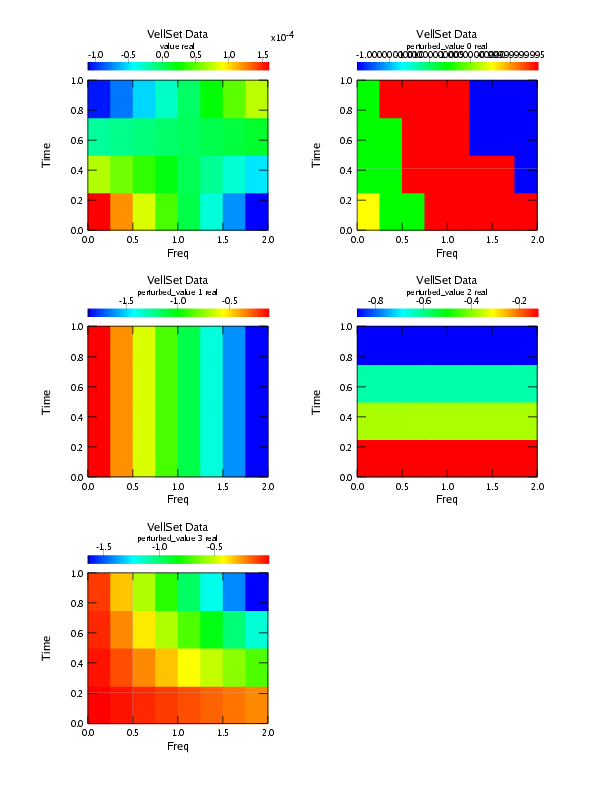
\includegraphics{Figures/condeq}}
\par}
\caption {The contents of the CondEq object after the glish script
has been run. These contents are discussed further 
in the text. Note: there is a bug somewhere in the plotting program -
all the values in the upper right image are the same: -1}
\label{fig:condeq}
\end{figure}
%\vspace{0.3cm}                         

At {\tt \#\#\#\# 10} we define various parameter for the MeqSolver object.
We tell the object that its child is the MeqCondeq node (`condeq'), that
we want to do 3 iterations for the solution of the equation parameters
and that the parameters that we are solving for are contained
in the MeqParm (`coeff') node. The actual MeqSolver node (`solver') is
then instantiated at {\tt \#\#\#\# 11}. 

At {\tt \#\#\#\# 12}  we use the `resolve' method to tell the nodes
to find their children if they have any.
Here, the solver is the starting node for
locating the positions of child nodes in the repository. Each
node downstream of the starting node will also find its children.
So, for example if we had said {\tt mqs.resolve('add')} we would only
have located children downstream of the `add' node.

This is a one time operation which needs to be done after the tree has been
defined.

\begin{figure}
{\par\centering
\resizebox*{0.9\columnwidth}{!}{\includegraphics{Figures/coeff}}
\par}
\caption {The contents of the MeqParm `coeff' object after the glish
script has been run. These contents are discussed further in the text.}
\label{fig:coeff}
\end{figure}

\begin{figure}
{\par\centering
\resizebox*{0.9\columnwidth}{!}{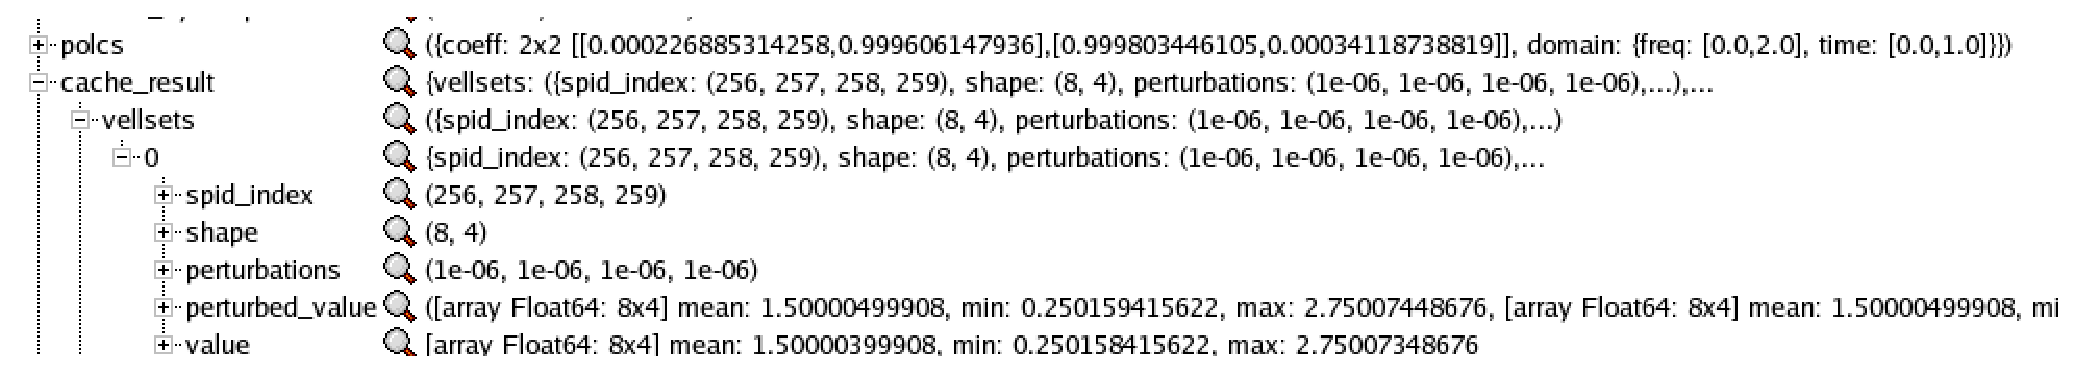
\includegraphics{Figures/coeff_polcs}}
\par}
\caption {The values of the Polcs array is shown in the top row of
this subsection of the `coeff' state record after the glish tree script
has been run.}
\label{fig:coeff_polcs}
\end{figure}


At {\tt \#\#\#\# 3} we specified the time and frequency ranges of the
domain. However until now our domain has not had any locations specified
where we will evaluate the function parameters we wish to solve for. We
remedy this situation by creating a {\tt cells} object at {\tt \#\#\#\# 13}.
We tell the system that we wish to break up the domain into 
4 frequency and 4 time cells. Note that the images we have shown so far
of contents of the MeqFreq, MeqTime and MeqAdd objects are generated while
the system is computing solutions - when these nodes were first 
instantiated we had not yet specified any {\tt cells} object, so these
objects could not yet contain an array.

%\vspace{0.3cm}
%\begin{figure}
%{\par\centering
%\resizebox*{1.0\columnwidth}{!}{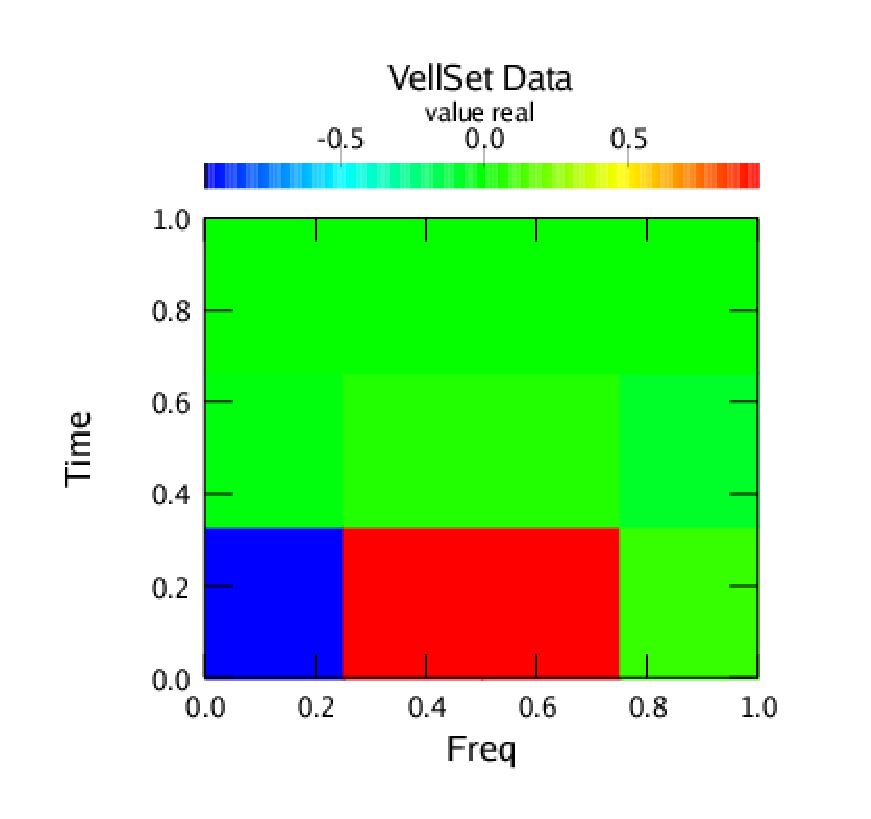
\includegraphics{Figures/solver1}}
%\par}
%\caption {The contents of the MeqSolver object after running the script. 
%These contents are discussed further in the text.}
%\label{fig:solver}
%\end{figure}
%\vspace{0.3cm}                         

At {\tt \#\#\#\# 14} we formulate a request for the MeqSolver object,
telling it we want to obtain a solution over the {\tt cells} that
we have specified, and that we only want to do first-order
perturbations (calc\_deriv=1).

Finally at {\tt \#\#\#\# 15} we tell the solver to execute the
request. 
The solver accumulates the condition equations from the Condeqs into
an N x M matrix, in which image N is the number of MeqParm coefficients
that are to be solved for by this solver. It then inverts the matrix
to obtain a least-squares solution which gives incremental improvements of
the solvable MeqParm parameter values. These increments are then added to the
MeqParm values, ready for the next iteration if there is one.

Figure ~\ref{fig:condeq} shows the contents of the MeqCondeq
node after we have run the glish tree script. There are five
images. The upper left one shows the final difference between
the results of its two children. Essentially we have quite
a good fit between the fitted and `observed' arrays 
as the differences are only of the order 0.0001. This image
always acts as the driving term in the condition equations
generated for the MeqSolver object. The remaining arrays
are actually perturbation arrays for each of the solvable
MeqParm coefficients in the order $a$, which should be constant,
$b$ - Frequency, $c$ - Time and $d$ - the $xy$ cross-term. These
are basically close approximations to the derivatives with respect to
each of the solvable MeqParm parameters. We perturb each parameter
by a small amount $\Delta x$ where $\Delta x$ is typically on
the order of $10^{-6}$.
The arrays actually represent $ (f(x+\Delta x) -f(x))/\Delta x$.

Figure ~\ref{fig:coeff} shows the contents of the MeqParm `coeff'
node after we have run the glish tree script. The upper left image
shows the final array as computed from the results of the polynomial
while the remaining images show the resulting images we get when
as a result of perturbing each of the four fitting parameters by 
the small perturbation value of $10^{-6}$ mentioned above.
In the present case these small perturbations have essentially
no effect on the output array so we can be fairly sure that our
fit result is reasonable.
 
We can find the final values of the coefficients for the polynomial
that we have computed by using Oleg Smirnov's `meqbrowser' program to look at
the contents of the nodes in the tree. After clicking on the `coeff' node
we can find the final results for our `Polc' array by looking at the 
`polcs' contents in the record for the `coeff' node - see 
Figure  ~\ref{fig:coeff_polcs}. The `polcs' contents include a `coeff' field
which lists out the final values of our four coefficients. 

In this section we showed the contents of various nodes in the 
tree after the glish script was run. These displays were obtained
by running the meqbrowser program. The next section gives a detailed
description of how to use this program.

\section{Display of Results}

The previous section showed the contents of MeqTree nodes in both 
image and record formats. We examine the contents of a tree
by running the `meqbrowser.py' script. When you start up this script
you will see a display similar to that shown in 
Figure  ~\ref{fig:browser1}. Probably the most important thing to
look for in this initial display is for a `running' statement in the
lower left hand corner. This tells you that the meqbrowser has
successfully connected to a meqserver and we will be able to view
the contents of nodes. If you see `no connection' you know you have a
problem, and you should shut down and restart the browser.

We are interested in examining the contents of tree nodes so, if the
browser status is `running', click on the `Trees' tab near the
bottom of the browser. You must then click on the `Update' icon
(the two arrows pointing at each other) in the upper left hand
corner of the display. This will give you a display that allows you
to look at nodes on the basis of `All Nodes', `By Class', or just 
the Root node at the base of the tree. 
We are interested in examining nodes by class so click
on the `+' sign next to `By Class', and you should see a display
similar to that shown in Figure  ~\ref{fig:browser2}. 

\begin{figure}
{\par\centering
\resizebox*{0.8\columnwidth}{!}{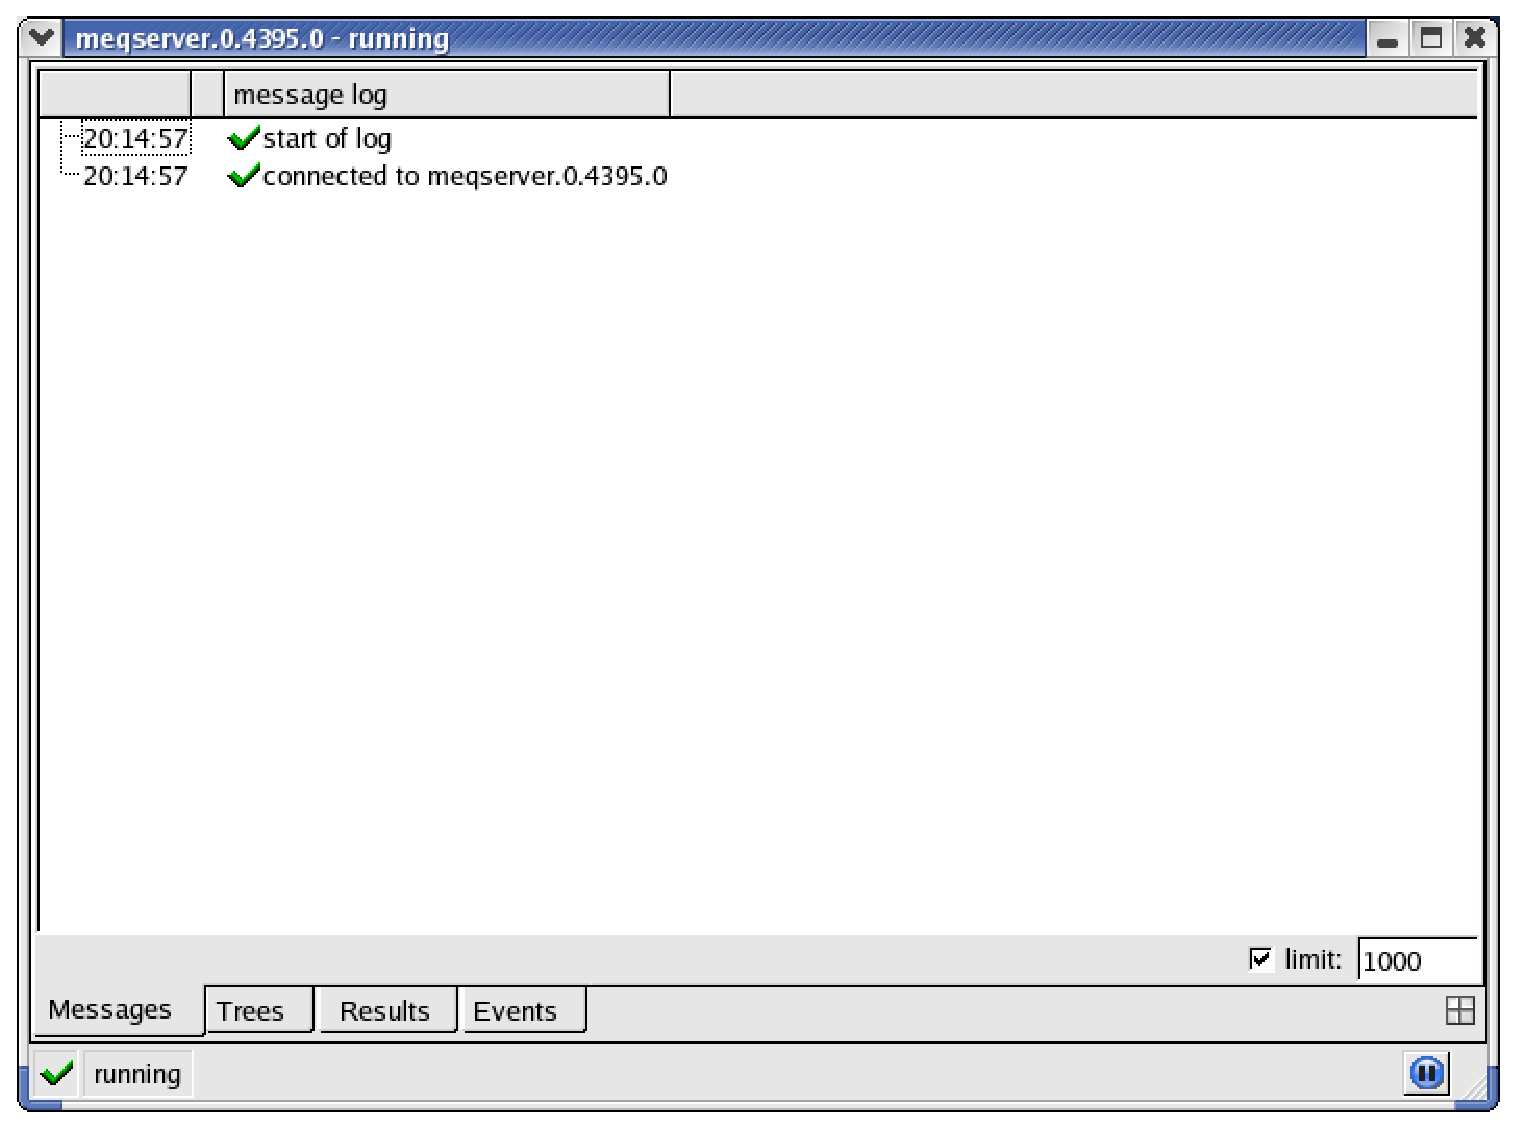
\includegraphics{Figures/browser1}}
\par}
\caption {The initial appearance of the browser after the user has 
started it with the meqbrowser.py script.}
\label{fig:browser1}
\end{figure}

\begin{figure}
{\par\centering
\resizebox*{0.8\columnwidth}{!}{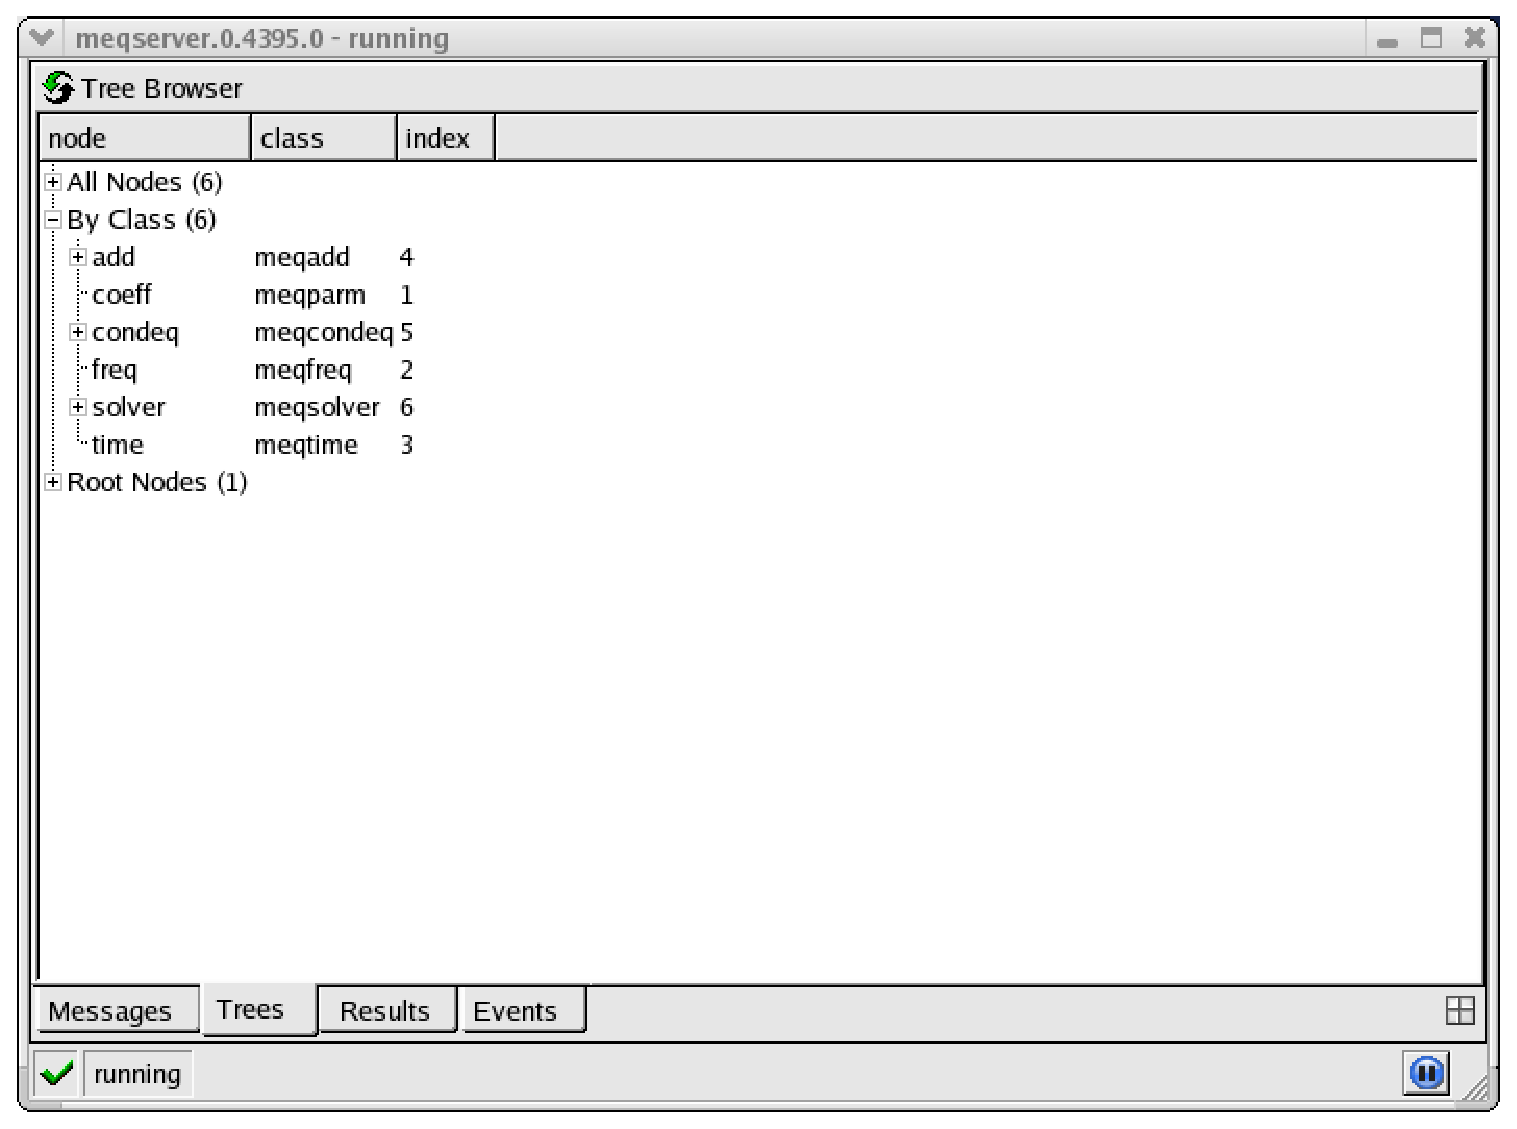
\includegraphics{Figures/browser2}}
\par}
\caption {The contents of the browser after the user has clicked on the
`Trees' tab at the bottom of the screen, then clicked on the 
`update Tree Browser' icon in the upper left hand corner, and finally
expanded the list of `class' nodes by clicking on the `+' icon next to
the `By Class' label in the nodes listing.}
\label{fig:browser2}
\end{figure}

Figure  ~\ref{fig:browser2} shows a list of nodes sorted by node type, or
class. One of the more interesting types of nodes to look at is the 
condeq (meqcondeq) node. If you click on `condeq' with the left mouse
button, the browser will give a detailed display of the contents of the
condeq's state record. This display is shown in Figure ~\ref{fig:browser3}.
The state record structure can give you some basic information about
the contents of a node, but in many cases you can get more information
by visualizing the contents of a node. Probably the most important
contents of a node are contained within the `cache\_result' sub-record.

Remember from our earlier discussion that the Condeq mode contains
a Vells, which is the difference between its two children and a
VellSet which contains the perturbed differences. If we right-click
on the cache\_result label, a context-sensitive menu will appear.
If you select the 'Result Plotter' option, a complete display of 
the Vells and perturbed results will appear in a separate GUI
display (see Figure ~\ref{fig:browser4}). We used selected contents
from this display to obtain the condeq display given in 
Figure  ~\ref{fig:condeq}.

\begin{figure}
{\par\centering
\resizebox*{0.8\columnwidth}{!}{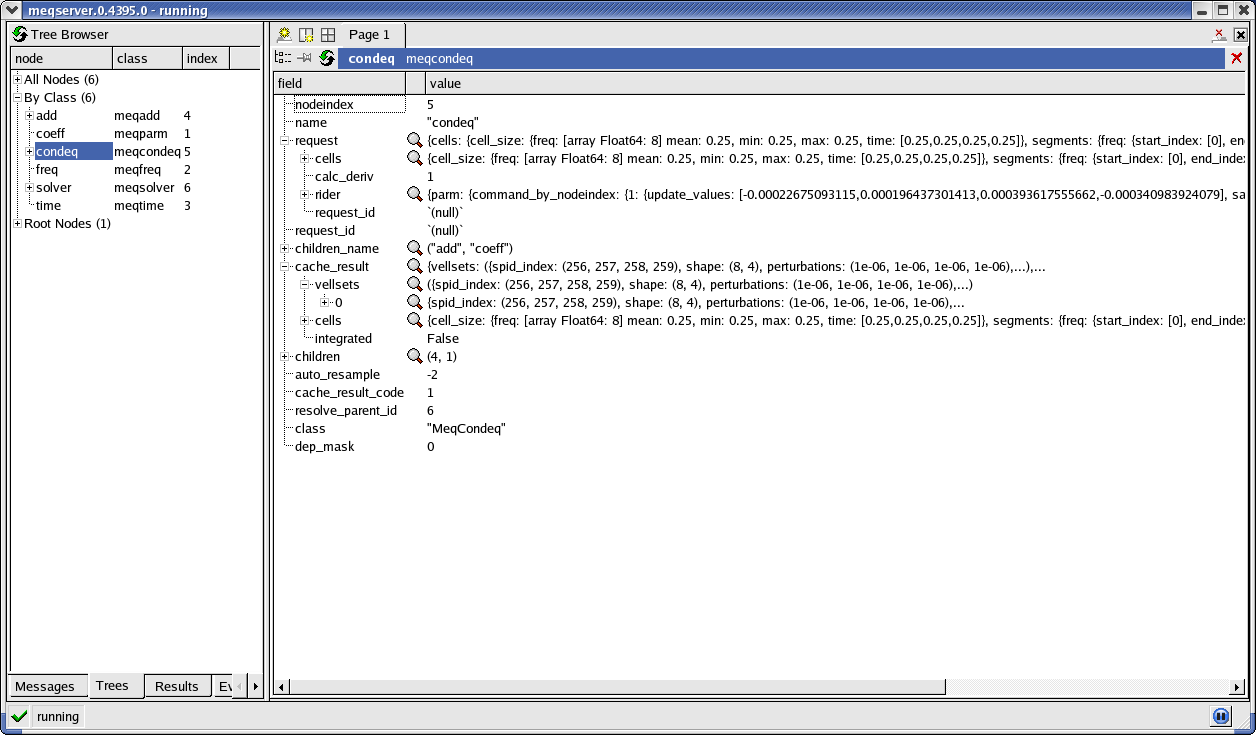
\includegraphics{Figures/browser3}}
\par}
\caption {The contents of the browser after the user has clicked on the
`condeq' label in Figure ~\ref{fig:browser2}. }
\label{fig:browser3}
\end{figure}

\begin{figure}
{\par\centering
\resizebox*{1.0\columnwidth}{!}{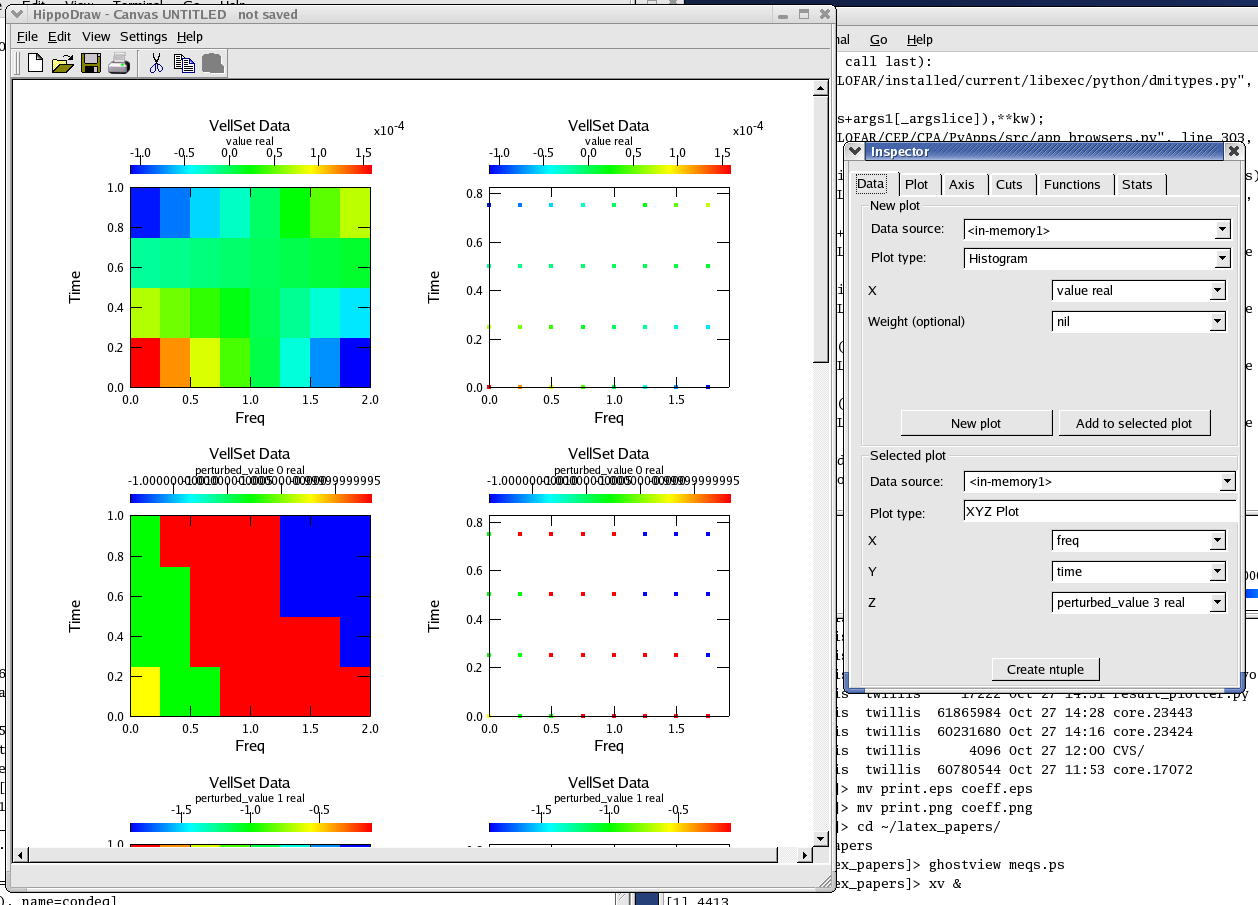
\includegraphics{Figures/browser4}}
\par}
\caption {The HippoDraw display that appears after the user
right clicks on the `cache\_result' label that can be seen in
Figure ~\ref{fig:browser3}, and then clicks on the `Result Plotter' option
of the drop-down menu that appears. The Inspector GUI is seen next to
the HippoDraw canvas.}
\label{fig:browser4}
\end{figure}

Sometimes you are interested in examining the contents of an individual
array, not the entire contents of a cache\_result. You can
do this if you left click on the `magnifying glass' next to an
array object. To access an array object you must be at the
node level where the contents of the array are defined. The example in
Figure ~\ref{fig:ArraySelect} shows you how to do this. The left
figure shows the contents of a cache\_result. We can expand the
contents of vellsets 0, by clicking on the `plus' sign next to the
0. By doing so we split up the contents into separate `shape' and `value'
labels. The contents of the `value' label begin with the word `array',
so you know that you are at the level where you can directly access
the contents of the array. Left clicking on the magnifying glass icon
next to the word `array' will cause a plot of the specified array
to appear. Although Figure ~\ref{fig:add} shows an array plot generated
by right clicking on a {\tt cache\_result} label, you would get a similar
result if you choose to get a plot by selecting an individual array.

You can directly view the numerical contents of an array by right-clicking
on an array label. This will cause a context menu to appear. Keeping
the right mouse button down, slide your mouse to the `Display with' option.
This will cause a new sub-menu to appear. Slide your mouse to the
`Array Browser' option and release the mouse. This will cause a
display similar to the one in  Figure ~\ref{fig:ArrayBrowser}
to appear. This display shows the numerical contents of the array
plotted in Figure ~\ref{fig:add}.


\begin{figure}
  \centering
  \begin{minipage}[c]{0.5\textwidth}
     \centering 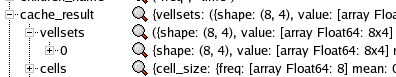
\includegraphics[width=2.5in]{Figures/browser_small1}
  \end{minipage}%
  \begin{minipage}[c]{0.5\textwidth}
     \centering 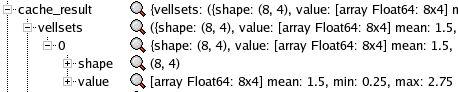
\includegraphics[width=2.5in]{Figures/browser_small2}
  \end{minipage}
  \caption {The browser display of (left) a cache\_result node, and 
(right) the expanded contents of this node after clicking on the
+ sign next to `0' under vellsets.}
  \label{fig:ArraySelect}
\end{figure}

\begin{figure}
{\par\centering
\resizebox*{0.8\columnwidth}{!}{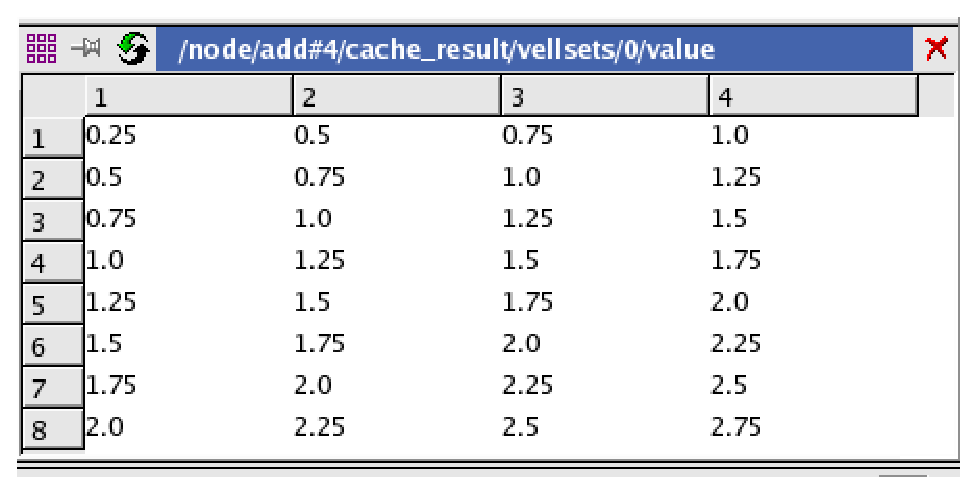
\includegraphics{Figures/array_browser}}
\par}
\caption {The numerical contents of an array that the browser shows
when one selects the `Array Browser' option. 
These contents are those of the array plotted in Figure ~\ref{fig:add}.}
\label{fig:ArrayBrowser}
\end{figure}

The display of 1 and 2-dimensional data is presently done with the
HippoDraw package written by Paul Kunz \cite{kunz}. The HippoDraw web 
page \cite{kunz} has
detailed instructions for its use. One of the attractions 
of HippoDraw is that once data has been loaded into it, it may be 
viewed in ways different from that seen in the default display
shown when the HippoDraw canvas first appears. You do so by making
use of the anciliary Inspector GUI shown in Figure  ~\ref{fig:Inspector} which
will appear next to the MeqBrowser GUI when you create 
the first HippoDraw display. Detailed instructions for using
the Inspector can be found at 
URL http://www.slac.stanford.edu/grp/ek/hippodraw/inspector\_root.html

When you click on one of the plots shown on the HippoDraw canvas,
that plot becomes the active plot, and the Inspector controls
refer to that plot. 
Even if you do not wish to make a new type of plot from the
data loaded into HippoDraw, two of the tabs on the Inspector, the
`Plot' and `Axis' tabs, allow you to interactively adjust many of the
parameters of the plot that has currently been selected, so you
should at least look at those two sections on the Inspector  
web page.

\begin{figure}
  \centering
  \begin{minipage}[c]{0.5\textwidth}
     \centering \includegraphics[width=2.2in]{Figures/inspector_top}
  \end{minipage}%
  \begin{minipage}[c]{0.5\textwidth}
     \centering \includegraphics[width=2.2in]{Figures/inspector_plot}
  \end{minipage}
  \caption {The HippoDraw Inspector GUI. The left picture shows the top
  level GUI. The right picture shows the contents of the `Plot' tab.}
  \label{fig:Inspector}
\end{figure}

You may end up making quite a bit of use of the `Plot' tab, shown
in the right part of Figure ~\ref{fig:Inspector}, that is contained within
the Inspector GUI. For instance, if the default Hippo plot shows data
in `image' format, as is the case for all the displays in this
document, you may turn the `image' plot into a contour map, by
first clicking on the `image' plot to select it, and then on the `Plot'
tab of the inspector. There, where the display says `Type', click on the 
`ColorBox' field. A pull down menu will appear; select `Contour' from
the pull-down menu, and the image display will be turned into a contour
map. Then you may modify the levels used for contouring, by clicking
on the `Axis' tab, and adjusting the parameters for contours in the
`Contour levels' box at the bottom of the `Axis' window.

An example of an image display and its corresponding contour representation is
shown in Figure ~\ref{fig:comparison}.


\begin{figure}
\begin{center}
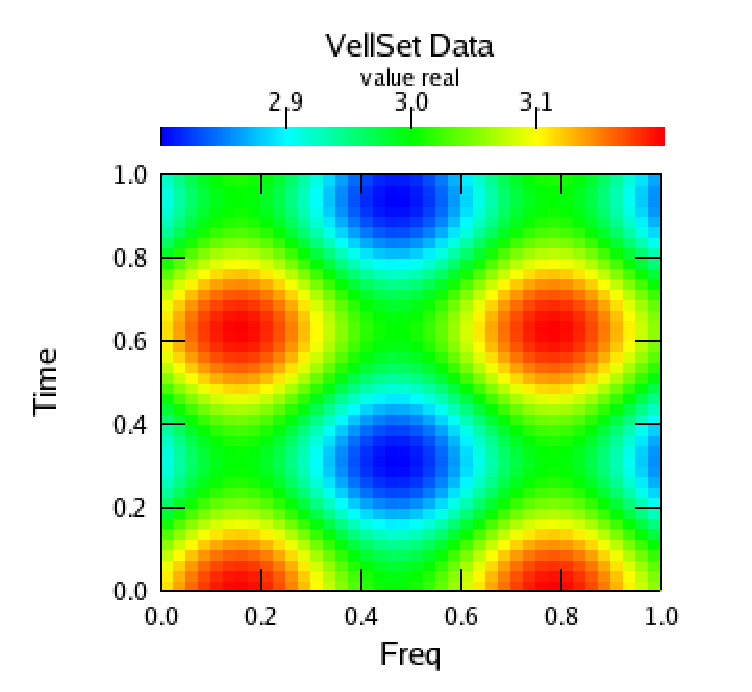
\includegraphics[width=2in]{Figures/image_display}
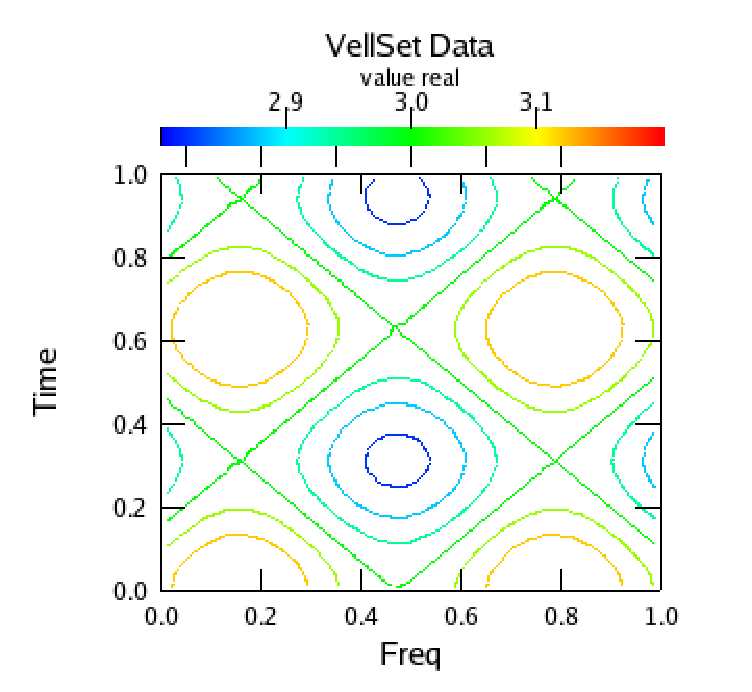
\includegraphics[width=2in]{Figures/contour_display}
\end{center}
\caption {A comparison of array data displayed in image form (left) 
and contour form (right) by HippoDraw.}
\label{fig:comparison}
\end{figure}

\vspace{1.0cm}                         
Acknowledgment: Thanks to Jan Noordam and Oleg Smirnov for guidance through 
the MeqForest!

\begin{thebibliography}{}
\bibitem{smirnov} Smirnov O.M., 2004, `MeqTree Kernel Design Overview (PSS4)',
ASTRON, Dwingeloo, the Netherlands
\bibitem{diepen} van Diepen G., 2003, `LOFAR Build Environment',
ASTRON, Dwingeloo, the Netherlands
\bibitem{kunz} Kunz, Paul, 2004, http://www.slac.stanford.edu/grp/ek/hippodraw
\end{thebibliography}
 
\appendix{Appendix}

\section {Installation instructions for PSS4}
This section is basically a verbatim copy of a set of instructions
written by Oleg Smirnov that describes the procedures for installing the 
packages and software necessary to run the PSS software system.
The PSS system is being developed inside the LOFAR build environment,
so many of the following instructions echo those given in the detailed
document written by Ger van Diepen \cite{diepen}.

\subsection{Prerequisites} 
  
\begin{verbatim}
  Current version numbers given; not guaranteed to work with earlier versions.
  (Most of this can be found on lofar9/10 under /usr/local/src.)

  Basic build:

    * Access to cvs.astron.nl. Read the LOFAR Build System document!

    * gcc-3.3.2 (not 3.4 yet!)

    * GNU toolset: automake 1.6.3, autoconf 2.53, libtool 1.5.2

    * A recent (post-library split) build of AIPS++

    * Blitz++ 0.6

    * log4cplus-1.0 

  Python meqbrowser (build/install in this order!)

    * Qt 3.3.2

    * Python 2.3.4

    * numarray-0.9 (Python package)

    * sip-4.0.1 (see http://www.riverbankcomputing.co.uk/pyqt/index.php)

    * PyQt-3.12

  For Tony's meqbrowser visualization plug-ins:

    * Boost-jam 3.1.10

    * Boost 1.31.0

    * Hippodraw 1.12
\end{verbatim}
  
\subsection{Installation notes for external packages}

\begin{verbatim}
  Generally, we build everything from source, and keep it under /usr/local. Look
  on lofar9/10 for an example layout. Configuration/build notes on specific
  packages:

  2.1. gcc-3.3.2 

  We configure it as follows:

  configure --prefix=/usr/local/gcc-3.3.2 
            --enable-threads=posix 
            --enable-version-specific-runtime-libs 
            --enable-languages=c,c++,f77
  make bootstrap && make install

  You may want to then set CC=/usr/local/gcc-3.3.2/bin/gcc and 
  CXX=/usr/local/gcc-3.3.2/bin/g++ in your environment, so that everything else
  is built with this compiler (this does matter for some of the packages!)

  2.2 GNU tools

  Configure with --prefix=/usr/local, and make sure that /usr/local/bin is first
  in your $PATH. Or just upgrade whatever version is in /usr.

  2.3. AIPS++ 

  As long as you've sourced aipsinit (i.e. your $AIPSPATH is set correctly),
  the LOFAR build system will figure everything else out.

  2.4. Blitz++

  ./configure --prefix=/usr/local/blitz/gnu3
  make && make install

  Blitz is somewhat sensitive to compilers, hence you need to keep different
  version if you use other compilers, the strange install path (the LOFAR build
  system will look for it there). Build it with gcc-3.3.2!

  2.5. log4cplus-1.0 

  ./configure --prefix=/usr/local
  make && make install

  2.6. Qt 3.3.2

  ./configure -thread -enable-opengl -prefix /usr/local/qt-3.3.2
  make && make install

  2.7 Python 2.3.4

  ./configure --prefix=/usr/local
  make && make install

  After make install, set /usr/bin/python to link to /usr/local/bin/python2.3.

  2.8. numarray-0.9 (Python package)

  See README. Run setup.py using the python built above, it should figure out the
  rest.

  2.9. sip, PyQt

  See README. Run configure.py using the python built above, it will figure out
  the rest.

  2.11. Hippodraw 1.12+.

  ./configure --prefix=/usr/local --enable-sipbuild --enable-numarraybuild
  --with-boost-include=/usr/local/boost-1.31.0/include/boost-1_31
  --with-boost-lib=/usr/local/boost-1.31.0/lib/ --with-Qt-dir=/usr/local/qt-3.3.2
  --with-Qt-lib=qt-mt
  
  ...was the easy part. As of 1.12.2, they still have a broken configure script,
  so you now need to set up some stuff by hand. Go into the ./sip subdirectory
  of the Hippo source tree, and look at the INSTALL file there. Specifically,
  you need to make sure that sip/Makefile contains:

      SIP = /usr/local/bin/sip
      PYQT_SRCS = -I /usr/local/share/sip -I /usr/local/share/sip/qtcanvas
      
  and finally, find the lines that look like:

      sipsihippocmodule.h : $(SIP_SRCS) 
	      @echo creating built sources
	      $(SIP) -e -g -c . $(PYQT_SRCS) -I $(top_srcdir)/sip  \
	      -t Qt_3_3_0 -t WS_X11 $(top_srcdir)/sip/sihippo.sip
  
  and make sure it says "Qt_3_3_0" for Qt-3.3.x (better check versions.sip
  too, just like the INSTALL file in sip instructs you).
  
  Now, back in the base of the Hippo source tree:
  make && make install
\end{verbatim}

\subsection {Checking out and building PSS4 per se}

\begin{verbatim}
  Assuming you have $CVSROOT set properly:

    :pserver:USERNAME@cvs.astron.nl:/cvs/cvsroot

  1. Start with 

    $ cvs login 
  # (persist until it logs you in)
    $ cvs co LOFAR/autoconf_share
    $ cvs up LOFAR/bootstrap
    $ cvs co LOFAR/LCS/Common
    $ cvs co LOFAR/DMI
    $ cvs co LOFAR/CEP/CPA
    # (the last one checks out a bunch of extra stuff under CEP/CPA that you
    # you don't really need. Delete later at your leisure. Only the following 
    # CEP/CPA packages are required for PSS4:
    #   OCTOPUSSY OCTOGlish OCTOPython GlishUtil VisCube AppAgent PSS4 PyApps

  2. Create the file LOFAR/lofarconf.in.private. This is just a list of packages
    to build, one per line (the default version, lofarconf.in, build the wrong 
    things). Use the following version:
    -------
       LCS/Common
       DMI
       CEP/CPA/OCTOPUSSY
       CEP/CPA/OCTOPython
       CEP/CPA/GlishUtil
       CEP/CPA/OCTOGlish
       CEP/CPA/VisCube
       CEP/CPA/AppAgent
       CEP/CPA/PSS4
       CEP/CPA/OCTOPython
       CEP/CPA/PyApps
    -------

  3. Create a variants file for your machine. Use variants.lofar10 as a 
    starting point.

    $ cd LOFAR/autoconf_share
    # this is assuming you're not on lofar10 to begin with.
    $ cp variants.lofar10 variants.YOUR_HOST_NAME

    Now check the variants file to make sure the compiler specification (CXX),
    Qt and aips++ paths all match your system. (Have no fear, if they don't, 
    you'll learn about it soon enough anyway).

    Note the use of "CXX=ccache\ /path/to/g++" in the file. This assumes you
    have ccache installed (and you should, it makes rebuilds a helluva lot 
    faster.) If you don't, just give the direct path to the compiler instead.

  3. Bootstrap the build environment, create build directory, configure:

    $ cd ~/LOFAR
    $ ./bootstrap
  # (watch messages go by...)

    $ mkdir -p build/gnu3_debug

    $ cd build/gnu3_debug
    $ ../../lofarconf
  # (watch messages go by...)
    $

    (Watch out here! One of the 'configures' called by the lofarconf script
    looks for a /aips++/weekly directory that contains a 'linux_gnu3' 
    directory. If your aips++ installation is set up differently, you 
    may have to set up some logical links to make the 'configure' happy.)

  4. Now, an evil but necessary kludge until I can get automake to submit:

    $ cd ~/LOFAR/CEP/CPA/OCTOPython/build/gnu3_debug/src
    $ ln -s octopython.la liboctopython.la

    (If you skip this step, PyApps will complain about a missing 
    liboctopython.la during the build.)

  5. Build!

    $ cd ~/LOFAR/build/gnu3_debug
    $ make 
  # (Go out to lunch)
    $

  5a. On lofar9/10, you may harness the awesome power of distcc and clustering, 
  to build at relativistic speeds on 20+ CPUs:

    $ mkdir ~/.distcc
  # copy over Oleg's distcc hosts file:
    $ cp ~oms/.distcc/hosts ~/.distcc
    $ export CCACHE_PREFIX=distcc    # this assumes bash, tcsh use setenv
    $ make -j40 
  # and hope it works...

  6. Installing the software.

    Assuming make was successful:

    $ cd ~/LOFAR/build/gnu3_debug
    $ make install

    This copies the built software and scripts into ~/LOFAR/installed/gnu3_debug.
    Handy for doing "snapshot"-style installs. 

  6a. Symlinking instead of installing

    A handy alternative is to set up a tree of symlinks directly into the
    source/build tree. Then, you never need to install, only edit/rebuild. I 
    recommend this approach if you're editing scripts, as it saves a lot of
    useless installs. 

    For an example symlink tree, see lofar10:/home/oms/LOFAR/installed/symlinked.
    You should be able to just copy Oleg's tree (since he uses relative symlinks) 
    and has everything working:

    $ slogin lofar10
    # (login)
    $ cd /home/oms/LOFAR/installed
    $ tar cvf ~/symlinks.tar symlinked.tar
    # (move the .tar file to your machine, and untar under your LOFAR/installed)

    Alternatively, you can copy them over directly, if you have access to his
    home directory locally. E.g., working on lofar9, you could do:

    $ cd ~/LOFAR/installed
    $ cp -a /net/lofar10/home/oms/LOFAR/installed/symlinked .

  7. Setting up include paths

    For Python, you need to set the $PYTHONPATH environment variable to

        $HOME/LOFAR/installed/current/libexec/python

    For Glish, just copy over Oleg's .glishrc from lofar10. 
    Or add the following to yours:

    #####
    system.path.include := [system.path.include,
      spaste(environ.HOME,'/LOFAR/installed/current/libexec/glish') ];

    lofar_software := [=];
    lofar_software.basepath := spaste(environ.HOME,'/LOFAR/installed/current');

    lofar_software.print_versions := T;

    lofar_software.gsm := [=];
    lofar_software.gsm.default_gsm_table := spaste(lofar_software.basepath,'/share/GSM/gsm.tab')

    lofar_software.meq := [=];
    lofar_software.meq.servers := [ './meqserver',spaste(lofar_software.basepath,'/bin/meqserver
    ####

    Note that this assumes that scripts and binaries may be found under
    ~/LOFAR/installed/current. 'current' should be set up as a symlink to
    whatever installation variant you actually want to use, i.e.,
    LOFAR/installed/gnu3_debug, or LOFAR/installed/symlinked.

  8. Some "simple" test trees

    To start the MEQ browser, run 
    LOFAR/installed/current/libexec/python/meqbrowser.py
    (or LOFAR/CEP/CPA/PyApps/src/meqbrowser.py, whichever's hanbier)

    In theory, you can just run leave the browser running permanently, as it
    connects/disconnects to the kernel automatically.

    To run a very simple test tree, go to 

    $ cd ~/LOFAR/CEP/CPA/PSS4/MeqServer/build/gnu3_debug

    First make some symlinks:

    $ ln -s ../../test/*.g .
    $ ln -s src/meqserver .

    Now you can run:

    $ glish -l ../../test/solver_test.g

    and then at the glish prompt (-) enter the line:

    solver_test(0)

    You can now watch sparks fly, and use the browser to examine the tree
    (if you don't see a tree, try clicking the refresh button at the top of the
    tree list).

  8a. When things go wrong(TM)

    The kernel is run in a process called 'meqserver'. This process will usually
    exit when you exit your glish session, but for reasons that are not yet 
    entirely clear, it may sometimes stay running in the background. Then, next
    time around you may end up with two running meqservers, at which point
    things get a little confusing for the browser. Someday Oleg will resolve this
    cleanly, but in the meantime,

    $ killall -9 meqserver

    is a useful incantation to know.

  9. meqsolve.g

    First make sure you are here:

    $ cd ~/LOFAR/CEP/CPA/PSS4/MeqServer/build/gnu3_debug

    Meqsolver.g solves for two sources in a Haystack simulated data set. To run
    meqsolve.g, you need to get a test measurement set. Get one here:

    lofar10:/home/oms/data-nobackup/haystack-ms/new_1_1/0128_vis_ninterp.MS

    and copy it some place you won't lose it... Now, set up another symlink:

    $ ln -s path/to/your/copy/of/test/measurement/set test.ms

    Now, you may run meqsolve.g. The '-filluvw' argument makes it populate the
    UVW tables first, you only need to give it _the very first time you use a
    particular MS_. It won't break things afterwards, but it's slow and useless
    to repeat the process.

    $ glish -l meqsolve.g -filluvw

    Everything else is controlled by editing meqsolve.g itself...
\end{verbatim}
     
\section{Creating Your Own Nodes }

Although it is unlikely that end users will want to create their
own specialized nodes, there may well be a requirement for a computer 
programmer to do so. Here are the instructions for a developer
to create his or her own Meq nodes inside the LOFAR environment.

\begin{verbatim}
Enter the directory where the source code for the nodes are kept:

   cd ~/LOFAR/CEP/CPA/PSS4/MeqNodes/src

Create the source code for the node (canabalize existing code):
create/edit <node>.cc and <node.h>
Add the <node>.cc file Makefile.am
Add the code to cvs:
   cvs add <node>.cc
   cvs add <node>.h

Enter the build directory:
   cd ~/LOFAR/CEP/CPA/PSS4/MeqNodes/build/gnu3_debug

Issue the command
   make aids (This will generate a global header file)

When you have created a new node class, you do a `make aids' to 
register the new type and allocate identifiers for
it. This regenerates a few source files, most notably
AID-MeqNodes.h, TID-MeqNodes.h, and AID-MeqNodes-Registry.cc 
in ~/LOFAR/CEP/CPA/PSS4/MeqNodes/src. 

Now, make sure that your code is up to date with regard to everyone 
else's check-ins.  A `cvs up' in CEP/CPA/PSS4/MeqNodes should be sufficient.
                                                                                
A rebuild is needed for MeqNodes, and all packages depending on it. But
if you do the make in ~/LOFAR/build/gnu3_debug, that should build
everything that's needs it.

So, to make and link with the LOFAR system:

cd ~/LOFAR/build/gnu3_debug

If you are on the LOFAR cluster you can do a parallel make by
issuing the command

   make -j40 

otherwise, just issue the command

   make

When you are sure that your new node works properly you should check in 
the regenerated files mentioned above along with the new node classes.

\end{verbatim}
\section {Code Maintenance and Dependency Issues} 
 
Oleg's advice on what to to if things are suddenly not building 
or not working: 

First of all, I've noticed the compiler crash randomly with an internal 
error. This has started happening since I've installed ccache and 
distcc. I'll look into the problem; in the meantime, I don't want to 
just disable these tools since they're saving an enormous amount of 
compilation time even despite the occasional glitches. So, if you see an 
internal error, just re-run make, it should be ok.

Now, if things are still truly screwed. If you just did a cvs up 
somewhere, then most likely you need to update some other package too. 
The full list of packages, in order of dependency, is as follows (also 
listed in LOFAR/lofarconf.in.private):

\begin{verbatim}
autoconf_share
LCS/Common
DMI
CEP/CPA/OCTOPUSSY
CEP/CPA/OCTOPython
CEP/CPA/GlishUtil
CEP/CPA/OCTOGlish
CEP/CPA/VisCube
CEP/CPA/AppAgent
CEP/CPA/PSS4
CEP/CPA/OCTOPython
CEP/CPA/PyApps
\end{verbatim}

Any time you do a checkout of some package, you
can check if something else under LOFAR/CEP/CPA needs updating by doing:
                                                                                
\begin{verbatim}
$ cd ~/LOFAR/CEP/CPA
$ cvs -n up        # if you want to be careful: -n option means show
what's new but do not modify any files
$ cvs up             # check out the updates
$ cd ~/LOFAR/build/gnu3_debug
$ make -j40      # rebuild
\end{verbatim}

Usually I just do a `cvs up LOFAR/CEP/CPA', to get all of CEP/CPA updated.
Very rarely, LCS/Common and DMI need an update too. If things still fail to
build then, it may be due to changes in the system build environment, or to
old libtool files (an unfortunate `feature' of the LOFAR build system). In
this case, try a complete clean:

\begin{verbatim}
$ cd LOFAR
$ cvs up autoconf_share
$ cd build/gnu3_debug
$ make distclean
$ cd ~/LOFAR
$ ./bootstrap
$ cd build/gnu3_debug
$ ../../lofarconf 
$ make -j40
\end{verbatim}


Note also the following cvs features:

- you can specify `cvs up -D $<$date$>$ package' to roll a specific package
back to a specific date. E.g. `cvs up -D yesterday' actually works as
expected.

One can get more specific with regard to date by doing e.g.

 cvs up -D `2004-07-11 20:05' package

- this operation places a `date tag' on that package, so it stays `frozen'
at the version checked out and ignores further updates. To reset it to the
most current version again, use `cvs up -A'.

- `cvs up' normally does not check out new directories, so if a package has
changed directory structure (very rarely, but happens), or if a new
directory is available, you have to use `cvs up -d'. Use this command with
discretion however: if you do a `cvs up -d' in LOFAR/CEP/CPA (or, worse yet,
in LOFAR), it will check out a zillion other packages that you really don't
want. Hence, you should only use it on a per-package basis.

- `cvs up -dPA' is the most `thorough' way to check out a package (but see
caution on using `d' above).
  
\end{document}
